\section{Quick Start: Reducing The Demo Data \label{sec:quick_start}}

For the user who is keen on starting reductions without being
distracted by detailed documentation, we describe the steps to be
performed to reduce the science data provided in the \instname\, demo
data set 
supplied with the {\tt Reflex~\reflexvers} release. By following these
steps, the user should have enough information to attempt a reduction
of his/her own data without any further reading:

\putgraph{8}{reflex_empty_canvas.png}{reflex_empty}{The empty {\tt
    Reflex} canvas}
\putgraph{14}{reflex_pipewkf_layout.png}{pipe_wkf_layout}{\instname\,
  workflow general layout}

%Esto estaba con \begin{figure}[htb]
\putgraph{6}{reflex_select_data_sets.png}{reflex_select_data_sets}{The
``Select Datasets'' pop-up window}

\begin{enumerate}
  \item Start the {\tt Reflex} application:
        \begin{verbatim}
        reflex &
        \end{verbatim}
        The empty {\tt Reflex} canvas as shown in Figure~\ref{fig:reflex_empty}
        will appear.

  \item Now open the \instname\, workflow by clicking on {\tt File -> Open
    File}, selecting first {\tt \pipename-\pipelinevers} and then the file {\tt
    \wkffilename} in the file browser.  You will be presented with the
    workflow canvas shown in Figure~\ref{fig:pipe_wkf_layout}. Note that
    the workflow will appear as a canvas in a new window.

  \item To aid in the visual tracking of the reduction cascade, it is advisable
  to use component (or actor) highlighting. Click on {\tt Tools -> Animate at
  Runtime}, enter the number of milliseconds representing the animation
  interval (100\,ms is recommended), and click \fbox{\tt OK}.

  \item Under ``Setup Directories'' in the workflow canvas there are
    seven parameters that specify important directories (green
    dots). Setting the value of {\tt ROOT\_DATA\_DIR} is the only
    necessary modification if you want to process data other than the
    demo data\footnote{If you used the install script {\tt
        install\_reflex}, then the value of the parameter {\tt
        ROOT\_DATA\_DIR} will already be set correctly to the
      directory where the demo data was downloaded.}, since
    the value of this parameter specifies the working directory within
    which the other directories are organised. Double-click on the
    parameter {\tt ROOT\_DATA\_DIR} and a pop-up window will appear
    allowing you to modify the directory string, which you may either
    edit directly, or use the \fbox{\tt Browse} button to select the
    directory from a file browser.  When you have finished, click
    \fbox{\tt OK} to save your changes.

  \item Click the 
  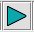
\includegraphics[width=0.5cm,height=0.5cm]{reflex_run_button.png}
  button to start the workflow

  \item The workflow will highlight the {\tt Data Organiser} actor
    which has recursively scanned the raw data directory (specified by the
    parameter {\tt RAWDATA\_DIR} under ``Setup Directories'' in the
    workflow canvas) and constructs the DataSets. Note that the
    calibration and reference data must be present either in {\tt
      RAWDATA\_DIR} or in {\tt CALIB\_DATA\_DIR}, otherwise DataSets
    may be incomplete and cannot be processed. However, if the same
    reference file was downloaded twice in different places this
    creates a problem as {\tt Reflex} cannot decide which one to use.

  \item The {\tt Data Set Chooser} actor will be highlighted next and
    will display a ``Select Datasets'' window (see
    Figure~\ref{fig:reflex_select_data_sets}) that lists the DataSets
    along with the values of a selection of useful header
    keywords\footnote{The keywords listed can be changed by
      right-clicking on the {\tt DataOrganiser} Actor, selecting {\tt
        Configure Actor}, and then changing the list of keywords in
      the second line of the pop-up window. Make sure that the {\tt
        Lazy Mode} is not active and then click on \fbox{\tt Commit}
      to save the change.}  namely the object name, grism and filter
    name, information about the slit/mask (INS.MASK.ID for MXU,
    INS.MOS.CHECKSUM for MOS, and INS.SLIT.NAME for LSS), binning, and
    detector name.  The first column consists of a set of tick boxes
    which allow the user to select the DataSets to be processed, and
    by default all DataSets are selected.

  \item Click the \fbox{\tt Continue} button and watch the progress of
    the workflow by following the red highlighting of the actors. A
    window will show which DataSet is currently being processed.

\end{enumerate}

Well done! You have successfully completed the quick start section and
you should be able to use this knowledge to reduce your own
data. However, there are many interesting features of {\tt Reflex} and
the \instname\, workflow that merit a look at the rest of this tutorial.
